\documentclass[12pt]{amsart}
% packages
\usepackage{graphicx}
\usepackage{setspace}
\usepackage{amssymb,amsmath,amsthm,amsfonts,amscd}
\usepackage{hyperref}
\usepackage{color}
\usepackage{booktabs}
\usepackage{tabularx}
\usepackage{enumitem}
\usepackage[retainorgcmds]{IEEEtrantools}
\usepackage[notref,notcite,final]{showkeys}
\usepackage[final]{pdfpages}
\usepackage{fancyhdr}
\usepackage{upgreek}
\usepackage{multicol}
\usepackage{fancyvrb}
\usepackage{listings}
% set margin as 0.75in
\usepackage[margin=0.75in]{geometry}

% tikz-related settings
\usepackage{tikz}
\usepackage{tikz-cd}
\usetikzlibrary{cd}

% theorem environments with italic font
\newtheorem{thm}{Theorem}[section]
\newtheorem*{thm*}{Theorem}
\newtheorem{lemma}[thm]{Lemma}
\newtheorem{prop}[thm]{Proposition}
\newtheorem{claim}[thm]{Claim}
\newtheorem{corollary}[thm]{Corollary}
\newtheorem{conjecture}[thm]{Conjecture}
\newtheorem{question}[thm]{Question}
\newtheorem{procedure}[thm]{Procedure}
\newtheorem{assumption}[thm]{Assumption}

% theorem environments with roman font (use lower-case version in body
% of text, e.g., \begin{example} rather than \begin{Example})
\newtheorem{Definition}[thm]{Definition}
\newenvironment{definition}
{\begin{Definition}\rm}{\end{Definition}}
\newtheorem{Example}[thm]{Example}
\newenvironment{example}
{\begin{Example}\rm}{\end{Example}}

\theoremstyle{definition}
\newtheorem{remark}[thm]{\textbf{Remark}}

% special sets
\newcommand{\A}{\mathbb{A}}
\newcommand{\C}{\mathbb{C}}
\newcommand{\F}{\mathbb{F}}
\newcommand{\N}{\mathbb{N}}
\newcommand{\Q}{\mathbb{Q}}
\newcommand{\R}{\mathbb{R}}
\newcommand{\Z}{\mathbb{Z}}
\newcommand{\cals}{\mathcal{S}}
\newcommand{\ZZ}{\mathbb{Z}_{\ge 0}}
\newcommand{\cala}{\mathcal{A}}
\newcommand{\calb}{\mathcal{B}}
\newcommand{\cald}{\mathcal{D}}
\newcommand{\calh}{\mathcal{H}}
\newcommand{\call}{\mathcal{L}}
\newcommand{\calr}{\mathcal{R}}
\newcommand{\la}{\mathbf{a}}
\newcommand{\lgl}{\mathfrak{gl}}
\newcommand{\lsl}{\mathfrak{sl}}
\newcommand{\lieg}{\mathfrak{g}}

% math operators
\DeclareMathOperator{\kernel}{\mathrm{ker}}
\DeclareMathOperator{\coker}{\mathrm{coker}}
\DeclareMathOperator{\image}{\mathrm{im}}
\DeclareMathOperator{\coim}{\mathrm{coim}}
\DeclareMathOperator{\rad}{\mathrm{rad}}
\DeclareMathOperator{\id}{\mathrm{id}}
\DeclareMathOperator{\hum}{[\mathrm{Hum}]}
\DeclareMathOperator{\eh}{[\mathrm{EH}]}
\DeclareMathOperator{\lcm}{\mathrm{lcm}}
\DeclareMathOperator{\Aut}{\mathrm{Aut}}
\DeclareMathOperator{\Inn}{\mathrm{Inn}}
\DeclareMathOperator{\Out}{\mathrm{Out}}
\DeclareMathOperator{\Gal}{\mathrm{Gal}}
\DeclareMathOperator{\End}{\mathrm{End}}


% frequently used shorthands
\newcommand{\ra}{\rightarrow}
\newcommand{\se}{\subseteq}
\newcommand{\ip}[1]{\langle#1\rangle}
\newcommand{\dual}{^*}
\newcommand{\inverse}{^{-1}}
\newcommand{\norm}[2]{\|#1\|_{#2}}
\newcommand{\abs}[1]{\lvert #1 \rvert}
\newcommand{\Abs}[1]{\bigg| #1 \bigg|}
\newcommand\bm[1]{\begin{bmatrix}#1\end{bmatrix}}
\newcommand{\op}{\text{op}}

% nicer looking empty set
\let\oldemptyset\emptyset
\let\emptyset\varnothing

\setlist[enumerate,1]{topsep=1em,leftmargin=1.8em, itemsep=0.5em, label=\textup{(}\arabic*\textup{)}}
\setlist[enumerate,2]{topsep=0.5em,leftmargin=3em, itemsep=0.3em}


% Jupyter Notebooks proramming stuff
\definecolor{codegreen}{rgb}{0,0.6,0}
\definecolor{codegray}{rgb}{0.5,0.5,0.5}
\definecolor{codepurple}{rgb}{0.58,0,0.82}
\definecolor{backcolour}{rgb}{1,1,1}

\lstdefinestyle{mystyle}{
    backgroundcolor=\color{backcolour},   
    commentstyle=\color{codegray},
    keywordstyle=\color{magenta},
    numberstyle=\tiny\color{codegray},
    stringstyle=\color{codegreen},
    basicstyle=\ttfamily\footnotesize,
    breakatwhitespace=false,         
    breaklines=true,                 
    captionpos=b,                    
    keepspaces=true,                 
    numbers=left,                    
    numbersep=5pt,                  
    showspaces=false,                
    showstringspaces=false,
    showtabs=false,                  
    tabsize=2
}

%box matrix
\newenvironment{boxmatrix}
    {
     \boxed{
     \begin{matrix}
            {
            }
     \end{matrix}}
    }

\lstset{style=mystyle}

\begin{document}
\begin{center}
    \textsc{Linear Algebra. HW III\\ Ian Jorquera\\ Colaborators:}
\end{center}
\vspace{1em}

\begin{itemize}
\item[(1)] For this problem I used Julia: to create the matrix I used 
\lstinputlisting[language=Python]{p1.jl}

Which gives us the following matrix

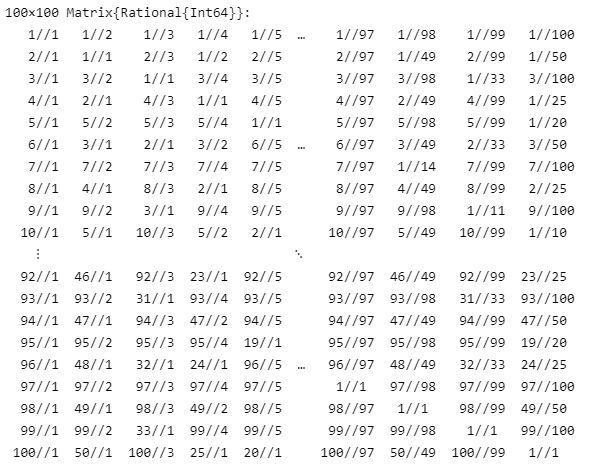
\includegraphics[scale=.6]{matp1.png}

We can then compute the null space using Julia's Linear Algebra library as shown below

\lstinputlisting[language=Python]{p2.jl}

Which gives us a matrix with $99$ columns representing the embedding map of the kernel whose dimension is $99$ into $\Q^{100}$

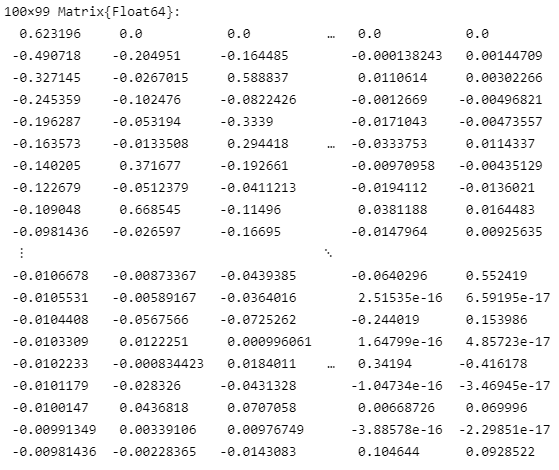
\includegraphics[scale=.6]{matp2.png}\\
\newpage
\item[(2)] Assume we have two solutions $\kernel_1\varphi$ and $\kernel_2\varphi$ to the kernel. That is we have the following commutative diagram.\\
\[
\begin{tikzcd}[row sep=1cm, column sep=.75cm]
W\arrow[leftarrow, rr, "\varphi"] & & V\\
& \kernel_1\varphi \arrow[d,"\hat\sigma"', bend right]\arrow[ul, "0"']\arrow[ur, hook, "\iota"']\\
& \kernel_2\varphi \arrow[uul, bend left, "0"]\arrow[u,"\sigma"', bend right]\arrow[uur, bend right, hook, "\nu"']
\end{tikzcd}
\]

We know that $\sigma$ exists uniquely by the kernelness of $\kernel_1\varphi$ and $\hat\sigma$ exists uniquely by the kernelness of $\kernel_2\varphi$.

We also know that by the kernelness of $\kernel_1\varphi$ that the identity map is the unique map that satisfies the follow diagram

\[
\begin{tikzcd}[row sep=1cm, column sep=.75cm]
W\arrow[leftarrow, rr, "\varphi"] & & V\\
& \kernel_1\varphi \arrow[ul, "0"']\arrow[ur, hook, "\iota"']\\
& \kernel_1\varphi \arrow[uul, bend left, "0"]\arrow[u,"\sigma\circ\hat\sigma"', bend right]\arrow[u,"id", bend left]\arrow[uur, bend right, hook, "\iota"']
\end{tikzcd}
\]

 But from the first diagram we also know that $\sigma\circ\hat\sigma$ also satisfies this diagram meaning $\sigma\circ\hat\sigma=\id_{\kernel_1\varphi}$. To see this more clearly we can chase the diagram: consider some $k\in \kernel_1\varphi$ we know that all paths must commute meaning $(\sigma\circ\hat\sigma)(k)=k$. 
 
 We also know that by the kernelness of $\kernel_2\varphi$ that the identity map is the unique map that satisfies the follow diagram

\[
\begin{tikzcd}[row sep=1cm, column sep=.75cm]
W\arrow[leftarrow, rr, "\varphi"] & & V\\
& \kernel_2\varphi \arrow[ul, "0"']\arrow[ur, hook, "\nu"']\\
& \kernel_2\varphi \arrow[uul, bend left, "0"]\arrow[u,"\hat\sigma\circ\sigma"', bend right]\arrow[u,"id", bend left]\arrow[uur, bend right, hook, "\nu"']
\end{tikzcd}
\]

 But from the first diagram we also know that $\hat\sigma\circ\sigma$ also satisfies this diagram meaning $\hat\sigma\circ\sigma=\id_{\kernel_2\varphi}$. So $\sigma$ and $\hat\sigma$ are both isomorphisms on the two kernels.\\% maybe mentions sigma is linear map.

\item[(3)] For any linear map $\varphi:V\ra W$ we will define the cokernel $\coker\varphi$ if there exists a linear map $\rho: W\twoheadrightarrow \coker\varphi$ such that $\rho\circ \varphi=0$ and for all $\kappa:W\twoheadrightarrow I$ satisfying $\kappa\circ \varphi=0$ there exists a unique linear map $\sigma:\coker\varphi\ra I$ such that the following diagram commutes.


\[
\begin{tikzcd}[row sep=1cm, column sep=.75cm]
W\arrow[leftarrow, rr, bend left, "\varphi"] & & V\\
& \coker\varphi \arrow[d, bend left, "\sigma"']\arrow[twoheadleftarrow, ul, "\rho"']\arrow[leftarrow, ur, bend left, "0"']\\
& I \arrow[twoheadleftarrow,uul, "\kappa"]\arrow[leftarrow, uur, bend right, "0"']
\end{tikzcd}
\]
% https://ctan.math.washington.edu/tex-archive/graphics/pgf/contrib/tikz-cd/tikz-cd-doc.pdf

In this case the cokernel tells us the elements that are not mapped to by $\varphi$ or the space of cosets that are parallel to the image. And so we need to require that the cokernel maps elements in the $\image\varphi$ to the zero coset(this is shown by the inner commutative triangle). Furthermore any other such space $I$ that satisfies this condition(shown by the outer triangle) needs to contain the cosets of the cokernel. This means $I$ may over quotient the space of $W$, mapping element of $W$ to zero when it is not needed, and the cosets of the cokernel need to uniquely factor into these larger cosets of $I$. This is shown by the arrow $\sigma$. Which is secretly a projection map of the coset of the cokernel into the cosets of $I$.\\

That is it may be the case that there exists some $w\in W$ such that $w\mapsto 0$ in $\kappa$ but $w\mapsto k\neq 0$ in $\rho$. This means that $\kappa$ quotients $W$ into larger cosets. If the arrow then goes up it would require $0\mapsto k$ in $\sigma$ in order to make the diagram commute. However this would break the commutative diagram and the zero arrow from $V$ to the cokernel would not commute. So the arrow must go down.\\ %Which tells us the imposter may map more then those required to $0$ and so the real cokernel would map exactly what is needed to zero and $\sigma$ would map all the extra element not mapped to zero. Another way to see this is that the set theory coker works here and is the best. It works because it does. But any $I$ would be of the form $W/U$ where $\image\varphi\se U\se W$ Meaning you would always have a (unique?) projection map from $W/\image\varphi$ to $W/\image\varphi/U/\image\varphi\cong W/U$. Basically what im getting at is that for the "real" cokernel any imposers would satisfy this diagram. It might be enough to just show that the set def satisfies this

\item[(4)] Ive been given the matrix 
\[
 \Phi=\boxed{\begin{matrix}
12 & 6 \\
14 & 32
\end{matrix}}
\]\\
I know very little about these numbers. But I know that I should probably do row reductions. First we can add $2$ times row $1$ to row $2$ to get
\[
 \boxed{\begin{matrix}
12 & 6 \\
-10 & 20
\end{matrix}}
\]\\

and then we can add row $2$ into row $1$ to get
\[
 \boxed{\begin{matrix}
2 & 26 \\
-10 & 20
\end{matrix}}
\]\\
and then we can add $5$ times row $1$ into row $2$ to find 
\[
 \boxed{\begin{matrix}
2 & 26 \\
0 & 150
\end{matrix}}
\]\\
From here we can see that our matrix has rank $2$ meaning the kernel must have dimension zero and so $J=0$ is the zero matrix.\\

\item[(5)] Consider the big matrix shown below

\[
 \boxed{\begin{matrix}
1   & 0 &   0 &   0 &   -1 &   -1 &    0 &    0 &    0\\
0   & 1 &   0 &   0 &    1 &    0 &   -1 &   -1 &    0\\
0   & 0 &   1 &   0 &    0 &    1 &    1 &    0 &   -1\\
0   & 0 &   0 &   1 &    0 &    0 &    0 &    1 &    1
\end{matrix}}
\]\\

We will start by exchanging the $7$nd column with the $3$th column, a basic column using row operations over the rationals. Here we will add the $3$st row to the $2$rd row to find that.

\[
 \boxed{\begin{matrix}
1   & 0 &   0 &   0 &   -1 &   -1 &    0 &    0 &    0\\
0   & 1 &   1 &   0 &    1 &    1 &   0  &   -1 &   -1\\
0   & 0 &   1 &   0 &    0 &    1 &    1 &    0 &   -1\\
0   & 0 &   0 &   1 &    0 &    0 &    0 &    1 &    1
\end{matrix}}
\]\\

Here we add row $2$ to row $1$ 

\[
 \boxed{\begin{matrix}
1   & 1 &   1 &   0 &    0 &    0 &    0 &   -1 &   -1\\
0   & 1 &   1 &   0 &    1 &    1 &   0  &   -1 &   -1\\
0   & 0 &   1 &   0 &    0 &    1 &    1 &    0 &   -1\\
0   & 0 &   0 &   1 &    0 &    0 &    0 &    1 &    1
\end{matrix}}
\]\\

Again We can repeat this by adding row $1$ to rows $2$ $3$ and $4$ to get that 

\[
 \boxed{\begin{matrix}
1   & 1 &   1 &   1 &    0 &    0 &    0 &    0 &    0\\
0   & 1 &   1 &   1 &    1 &    1 &   0  &    0 &    0\\
0   & 0 &   1 &   1 &    0 &    1 &    1 &    1 &    0\\
0   & 0 &   0 &   1 &    0 &    0 &    0 &    1 &    1
\end{matrix}}
\]\\

Now we will subtract row 1 from all other rows to get 

\[
 \boxed{\begin{matrix}
1   & 1  &   1 &   1 &    0 &    0 &    0 &    0 &    0\\
-1  &  0 &   0 &   0 &    1 &    1 &   0  &    0 &    0\\
-1  & -1 &   0 &   0 &    0 &    1 &    1 &    1 &    0\\
-1  & -1 &  -1 &   0 &    0 &    0 &    0 &    1 &    1
\end{matrix}}
\]\\


At which point all $4$ of the basic columns have been exchanged such that they are no longer in their originally positions.

\end{itemize}

\end{document}


